\documentclass[12pt]{article}
%Gumm{\color{blue}i}|065|=)
\usepackage{amsmath, amsfonts, amssymb}
\usepackage[margin=0.5in]{geometry}
\usepackage{xcolor}
\usepackage{graphicx}

% zeta funct{\color{blue}i}ons of cub{\color{blue}i}c f{\color{blue}i}elds

%\usepackage{p{\color{blue}i}font}
\usepackage{amsmath}

\newcommand{\off}[1]{}
\DeclareMathSizes{20}{30}{20}{18}

\newcommand{\two }{\sqrt[3]{2}}
\newcommand{\four}{\sqrt[3]{4}}





\usepackage{tikz}

\newcommand{\susy}{{\bf Q}}
\newcommand{\RV}{{\text{R}_\text{V}}}

\title{Scratchwork: Diffeomorphism of the Disk}
\date{}
\begin{document}

%\fontfam{\color{blue}i}ly{qag}\selectfont \fonts{\color{blue}i}ze{12.5}{15}\selectfont

\sffamily

\maketitle

\noindent The disc $D^2 = \{ x^2 + y^2 < 1 \}$ is fancy name for the inside of a circle.  But this is a proxy for the inside of any shape however complicated\dots In cartography, the shape of a country or a state, or county has is a \textbf{polygon} with thousands of sides.  Even a \textbf{multi-polygon}.  However, we do not have time to draw all of these. How can we accurately describe the shape without losing too much information. \\ \\
So now we must bicker about these words ``accurately" and ``shape".  Even the word ``too much" is going to be a point of controversy.  I will pick a definition, and you will pick a definition and they will slightly disagree.  \\

\noindent \includegraphics[width=0.75\textwidth]{subway-01.png} \\

\noindent So diffeomorphism is just a way to change one map to another without any ``errors" or ``singularities".  A polygon is just a circle.  So any diffeomorphism is really just a map from a circle to itself.   \\ \\
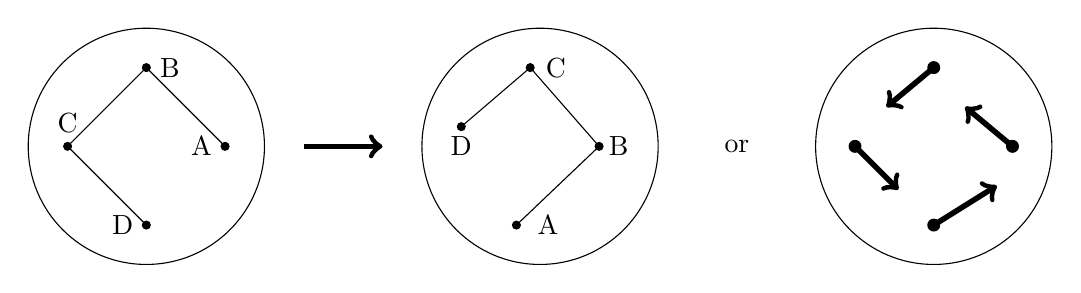
\begin{tikzpicture}

\begin{scope}
\draw (0,0) circle (1.5);

\draw[fill=black] (1,0) circle (0.05);
\draw[fill=black] (0,1) circle (0.05);
\draw[fill=black] (-1,0) circle (0.05);
\draw[fill=black] (0,-1) circle (0.05);

\draw (1,0)--(0,1)--(-1,0)--(0,-1);

\node at (0.7,0) {A};
\node at (0.3,1) {B};
\node at (-1,0.3) {C};
\node at (-.3,-1) {D};

\draw[->, line width = 2] (2,0)--(3,0);

\end{scope}

\begin{scope}[xshift=5cm]
\draw (0,0) circle (1.5);

\draw[fill=black] (0.75,0) circle (0.05);
\draw[fill=black] (-0.125,1) circle (0.05);
\draw[fill=black] (-1,0.25) circle (0.05);
\draw[fill=black] (-0.3,-1) circle (0.05);

\draw (-0.3,-1)--(0.75,0)--(-0.125,1)--(-1,0.25);

\node at (0.1,-1) {A};
\node at (1,0) {B};
\node at (0.2,1) {C};
\node at (-1,0) {D};

\node at (2.5,0) {or};

\end{scope}

\begin{scope}[xshift=10cm]
\draw (0,0) circle (1.5);


\draw[fill=black] (1,0)  circle (0.075);
\draw[fill=black] (0,1)  circle (0.075);
\draw[fill=black] (-1,0) circle (0.075);
\draw[fill=black] (0,-1) circle (0.075);

\draw[->, line width = 2] (1,0)--(0.4,0.5);
\draw[->, line width = 2] (0,1)--(-0.6,0.5);
\draw[->, line width = 2] (-1,0)--(-0.45,-0.55);
\draw[->, line width = 2] (0,-1)--(0.8,-0.5);

\end{scope}
\end{tikzpicture}

Turning these cartoons into a real map, or dually reducing an overly complicatd (i.e. ``realistic map") into something readable, requires some math.  We need a map:
$$ f: \mathbb{R}^2 \to \mathbb{R}^2 \text{ and } Df = \left[ \begin{array}{cc}
\frac{\partial f_1}{\partial x} & \frac{\partial f_1}{\partial y}  \\ 
\frac{\partial f_2}{\partial x} & \frac{\partial f_2}{\partial y}  \end{array} \right] $$
The derivative of a function from the plane to itself (a ``vector field") is now a $2 \times 2$ matrix.  And the surface is not-quite-flat.  So there might be a curvature terms\dots Nonetheless we can reduce much of this to nearly calculus, just a little bit more. \\ \\ 
We could draw $n = 4$ points or $n = 10^6$ points -- millions of data points -- can we still complete this map to a $C^\infty$ diffeomorphism, with a formula?  Taylor's theorem.
$$ f(x + dx, y+dy) \approx f(x,y) +  Df \cdot (dx,dy)  + O(|Df|^2)$$
and what is the margin of error?  This becomes a job for the mean value theorem.  To conclude for now:
$$ \big[\text{simplify a map}\big] \to \big[\text{mean value theorem}\big] $$
Even with four data points, we could get the behavior near by and near the limiting boundary circle.  In the city, there are soures and sinks to places far far away.  These could also be incorporated into our model.  \\ \\
\begin{minipage}{0.5\textwidth}
\begin{tikzpicture} 
\begin{scope}
\draw(0,0)--(2,0)--(2,2)--(0,2)--cycle;

\draw[->, line width = 2] (3,1)--(4,1);
\end{scope}

\begin{scope}[xshift=5cm]
\draw(0,0)--(2,0)--(2,1)--(1,1)--(1,2)--(0,2)--cycle;
\end{scope}

\end{tikzpicture}
\end{minipage}
\begin{minipage}{0.5\textwidth}
There's too much freedom still when we say ``diffeomorphism" so we can preserve distances somewhat and still get a decent map.  Show me a map from the $\square$ to the $\textbf{L}$ shape?
\end{minipage} \\ \\
\noindent The \textbf{Riemann mapping theorem} ensures us the existince of such a map, but doesn't tell us in any way how to get there.  We make bail.
\vfill

\begin{thebibliography}{}

\item Artur Avila, Sylvain Crovisier, Amie Wilkinson
\textbf{Diffeomorphisms with positive metric entropy} \texttt{arXiv:1408.4252}

\item F. Ledrappier and L.-S. Young \textbf{The metric entropy of diffeomorphisms} \\ Bull. Amer. Math. Soc. (N.S.), Volume 11, Number 2 (1984), 343-346.

\item Jacob Kastrenakes. \textbf{Circular subway map reimagines New York as a colorful, geometric array} \texttt{https://www.theverge.com/2013/7/29/4569204/max-roberts-circular-nyc-subway-map-redesign} \\
\texttt{http://gothamist.com/2013/07/25/fun\_map\_nyc\_subway\_map\_as\_a\_circle.php} \\
\texttt{http://gothamist.com/2018/05/03/vignelli\_subway\_map\_circles.php}

\item William L. Burke.  \textbf{Applied Differential Geometry} Cambridge University Press, 2012.

\end{thebibliography}
\end{document}